\exercise{Spatial filtering}
\subsection*{a - Convolution}
Spatial filtering is an operation where each pixel is changed based on the values of the pixels in its neighborhood.
By performing these kinds of operations, interesting operations like blurring, sharpening or edge detection can be performed that are not possible with simple pointwise operations.

When performing spatial filtering on an image it is usually defined how a pixel is influenced by its neighborhood.
This definition is usually in the form of a matrix, which is called the mask or kernel.
By applying the mask to each pixel, a spatial filtered result is be obtained.
By iterating over the pixels in the image, and applying the mask to every pixel's neighborhood, one can retrieve an enhanced image.
This process is called convolution.

We have implemented this operation in the following Matlab code: 

\matlabexternal{IPfilter.m}

This function can convolute any image with a mask of any odd size.
To test that it behaves correctly we have applied a Gaussian kernel (as in Table~\ref{tbl:gauss}) to an image, which should result in a blurred version of the image.
Figures~\ref{fig:nonblur} and~\ref{fig:blur} illustrate the result.
\begin{figure}[!htb]
 \centering
 \begin{subfigure}[b]{0.49\linewidth}
  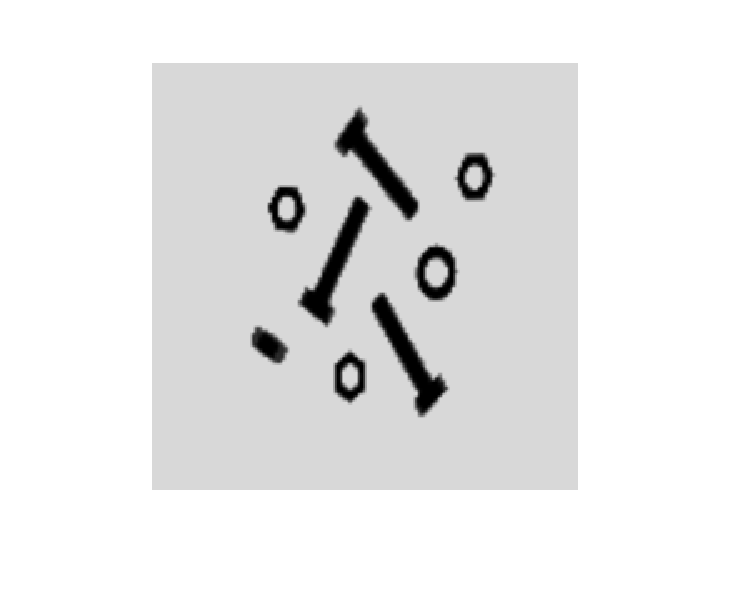
\includegraphics[width=\textwidth]{notBlurred.eps} 
  \caption{An image which was not blurred}
  \label{fig:nonblur} 
 \end{subfigure}
 \begin{subfigure}[b]{0.49\linewidth}
  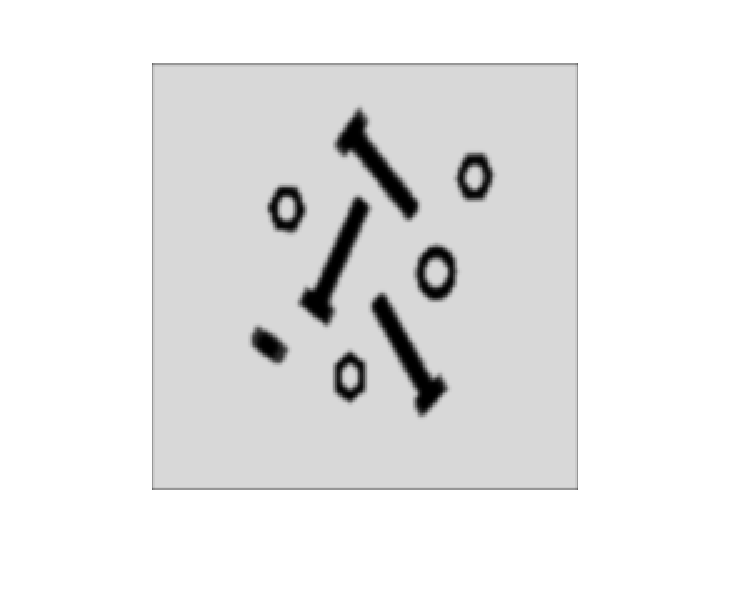
\includegraphics[width=\textwidth]{blurred.eps}
  \caption{The same image convoluted with a \(5 \times 5\) Gaussian kernel}
  \label{fig:blur}
 \end{subfigure}
 \caption{Gaussian mask applied to an image to demonstrate convolution}
\end{figure}
\begin{table}[!htb]
\begin{center}
$\frac{1}{273}$
\begin{tabular}{|c|c|c|c|c|}\hline
1 & 4 & 7 & 4 & 1\\ \hline
4 &  16 &  26 &  16 &  4 \\ \hline
7 &  26 &  41 &  26 &  7\\ \hline
4 &  16 &  26 &  16 &  4\\ \hline
1 &  4 &  7 &  4 &  1 \\ \hline
\end{tabular}

\caption{Gaussian kernel for blurring}
\label{tbl:gauss}
\end{center}
\end{table}
